<<<<<<< HEAD
%!TEX root = ../thesis-guntur.tex
=======
>>>>>>> deb4eee798046ff3050e2fdc49aff179daa28237
%********************************************************************
% Appendix
%*******************************************************
% If problems with the headers: get headings in appendix etc. right
%\markboth{\spacedlowsmallcaps{Appendix}}{\spacedlowsmallcaps{Appendix}}
<<<<<<< HEAD
\chapter{Access Point Count Correlation}
\label{ch:appendix-sensor-readings}

\section{Scatter Plots} % (fold)
\label{sec:scatter-plots}
% ap vs head count
\begin{figure}[H]
  \begin{adjustwidth}{-1cm}{}
  \centering
  \subfloat[day 1]{
    \label{fig:ap-hc-day1}{
      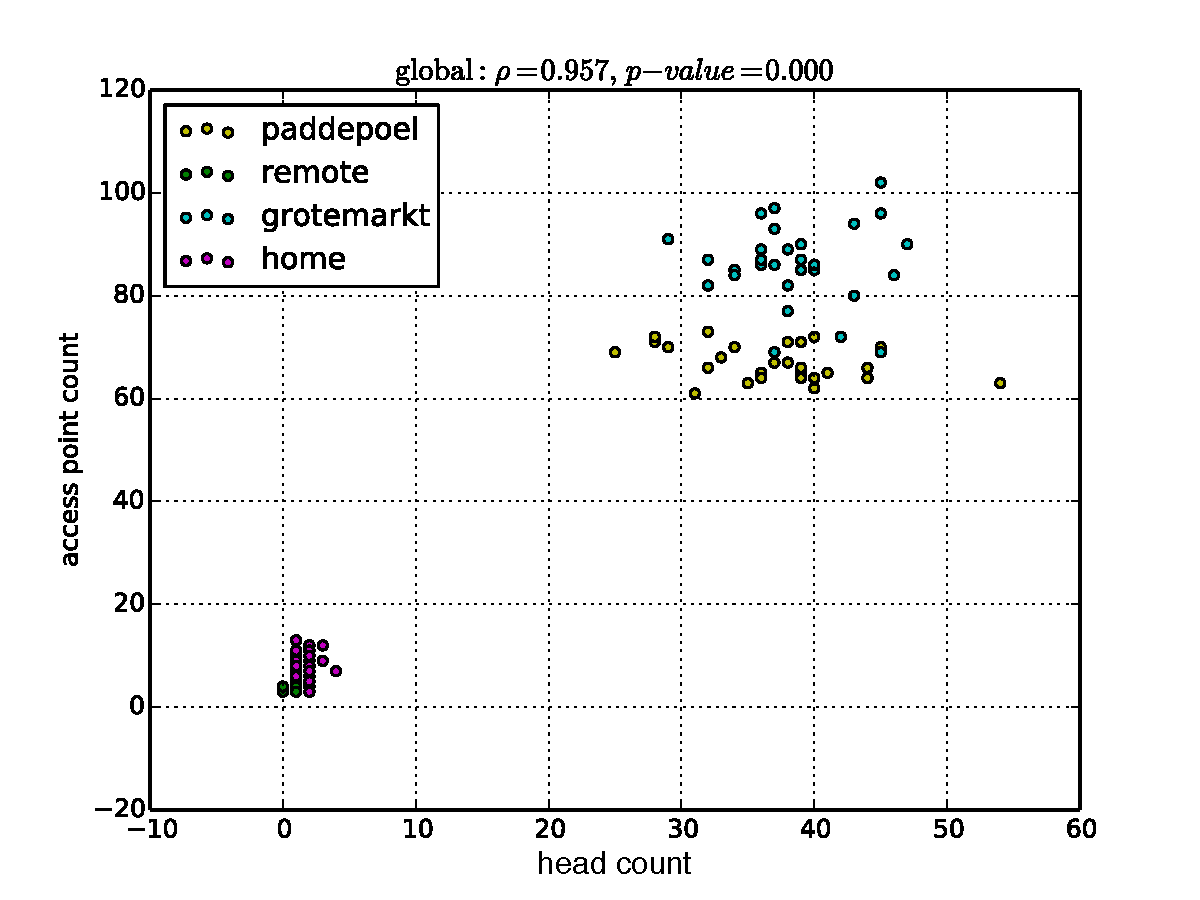
\includegraphics[width=0.7\textwidth]{./img/result/day/day1/global-gt-vs-ap}
    }
  }
  \subfloat[day 2]{
    \label{fig:ap-hc-day2}{
      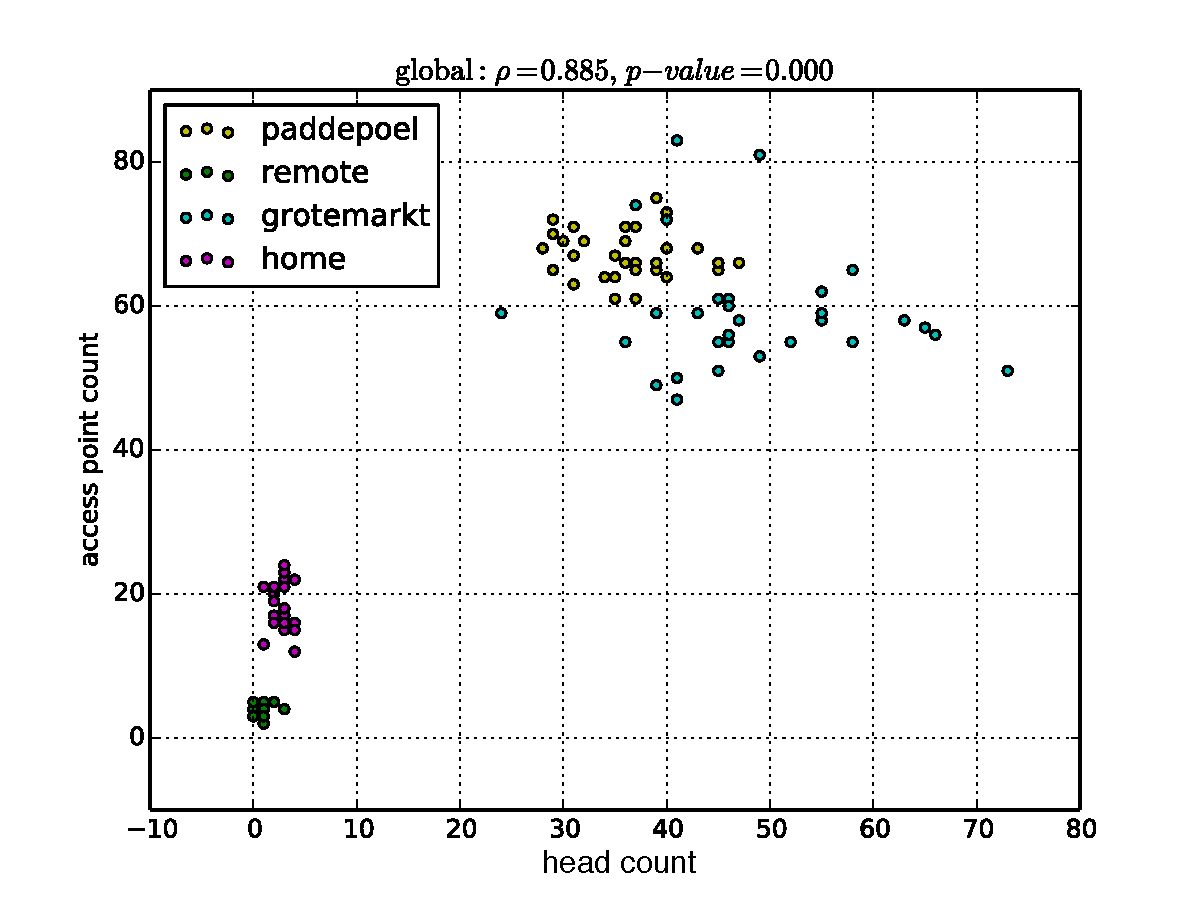
\includegraphics[width=0.7\textwidth]{./img/result/day/day2/global-gt-vs-ap}
    }
  }\\
  \subfloat[day 3]{
    \label{fig:ap-hc-day3}{
      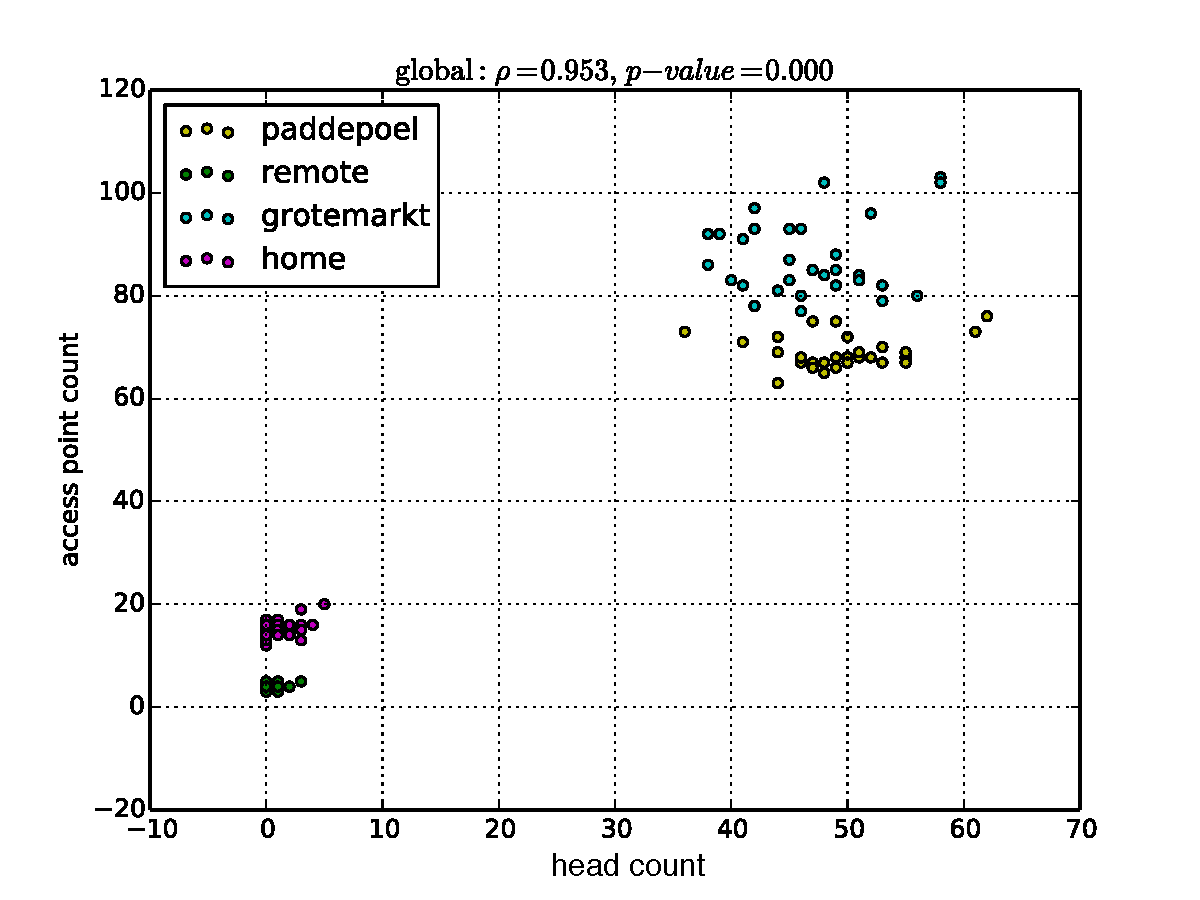
\includegraphics[width=0.7\textwidth]{./img/result/day/day3/global-gt-vs-ap}
    }
  }
  \subfloat[day 4]{
    \label{fig:ap-hc-day4}{
      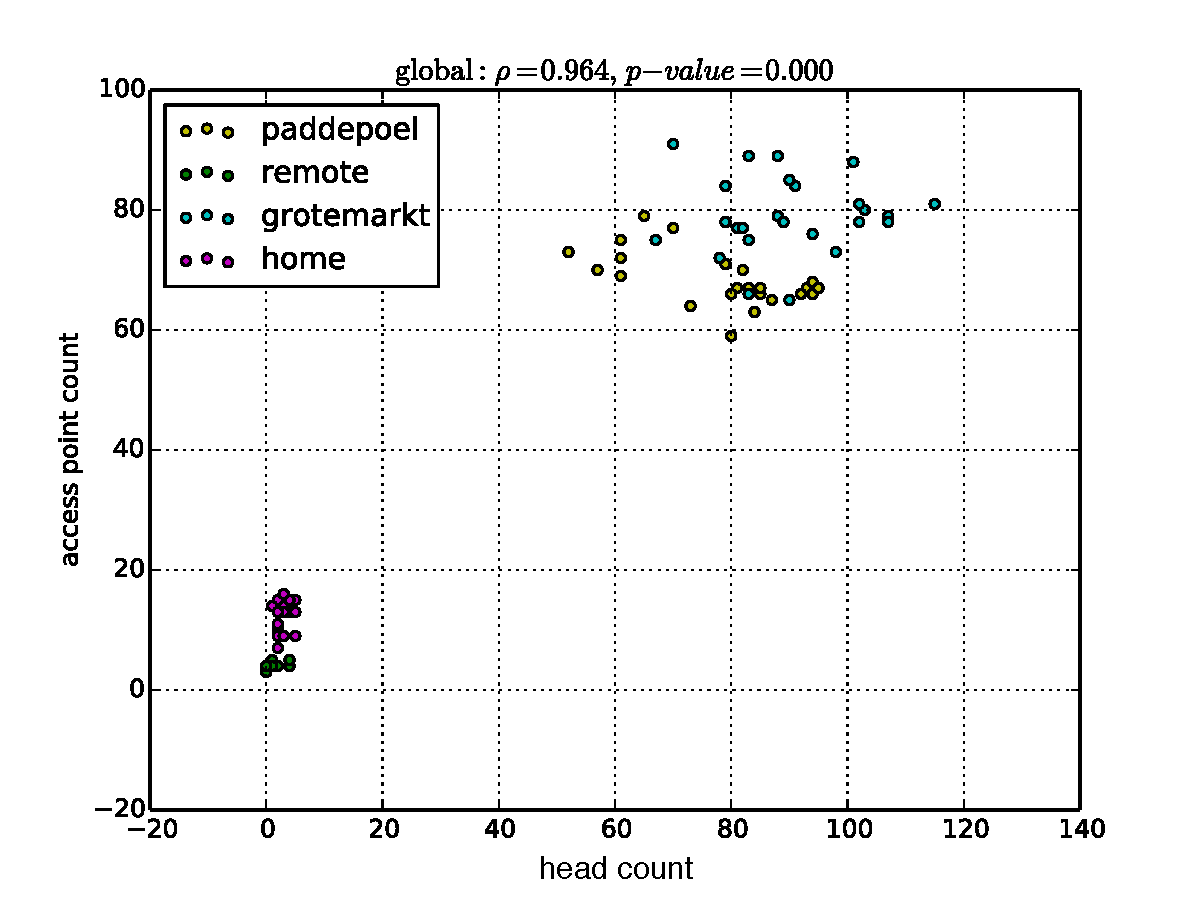
\includegraphics[width=0.7\textwidth]{./img/result/day/day4/global-gt-vs-ap}
    }
  }
  \end{adjustwidth}
  \caption[The scatter plots of the correlation between headcount and \ac{AP} count.]
  {The scatter plots showing the correlation between headcount and \ac{AP} count in four days of experiment. The location is coded in color.}
  \label{fig:ap-hc-scatterplot}
\end{figure}

% ap vs device count
\begin{figure}[H]
  \begin{adjustwidth}{-3cm}{}
  \centering
  \subfloat[day 1]{
    \label{fig:ap-dc-day1}{
      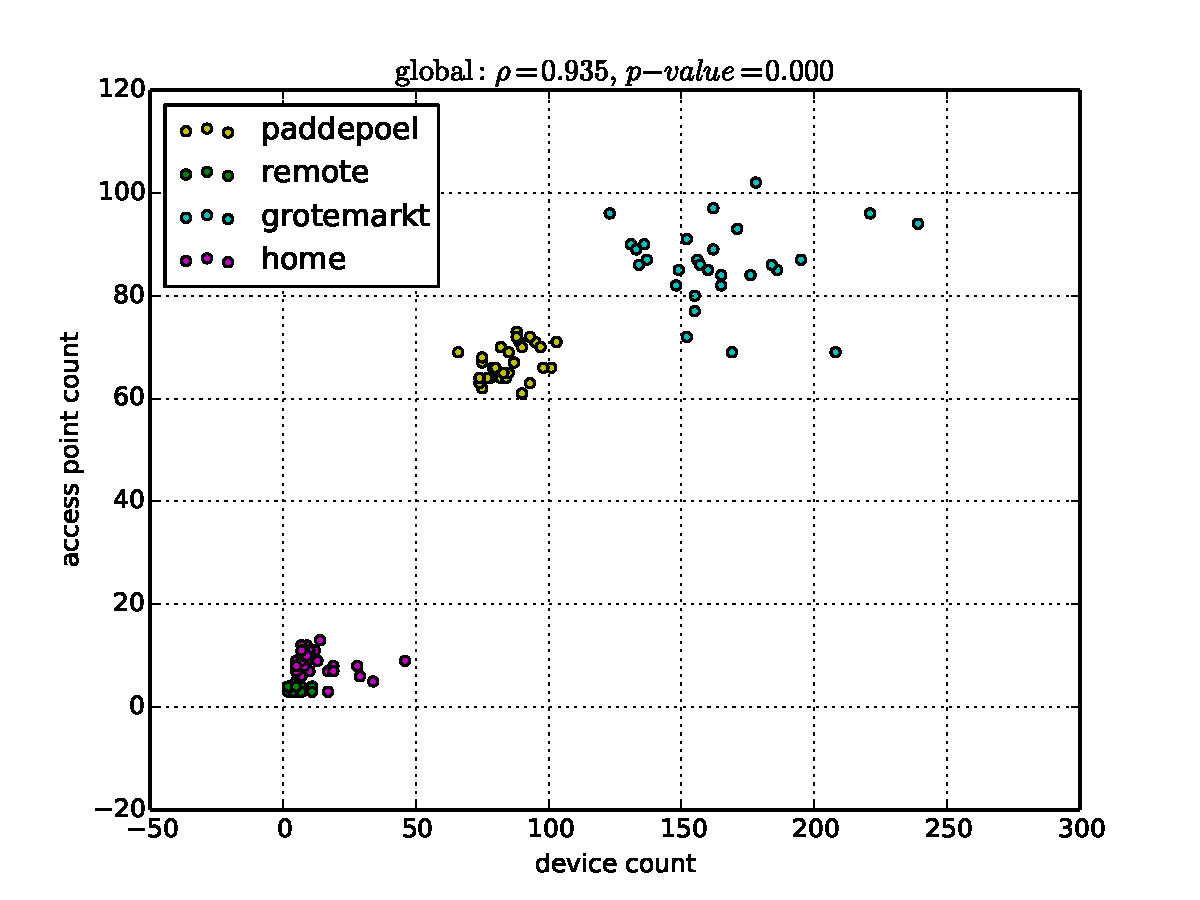
\includegraphics[width=0.7\textwidth]{./img/result/day/day1/global-pr-vs-ap}
    }
  }
  \subfloat[day 2]{
    \label{fig:ap-dc-day2}{
      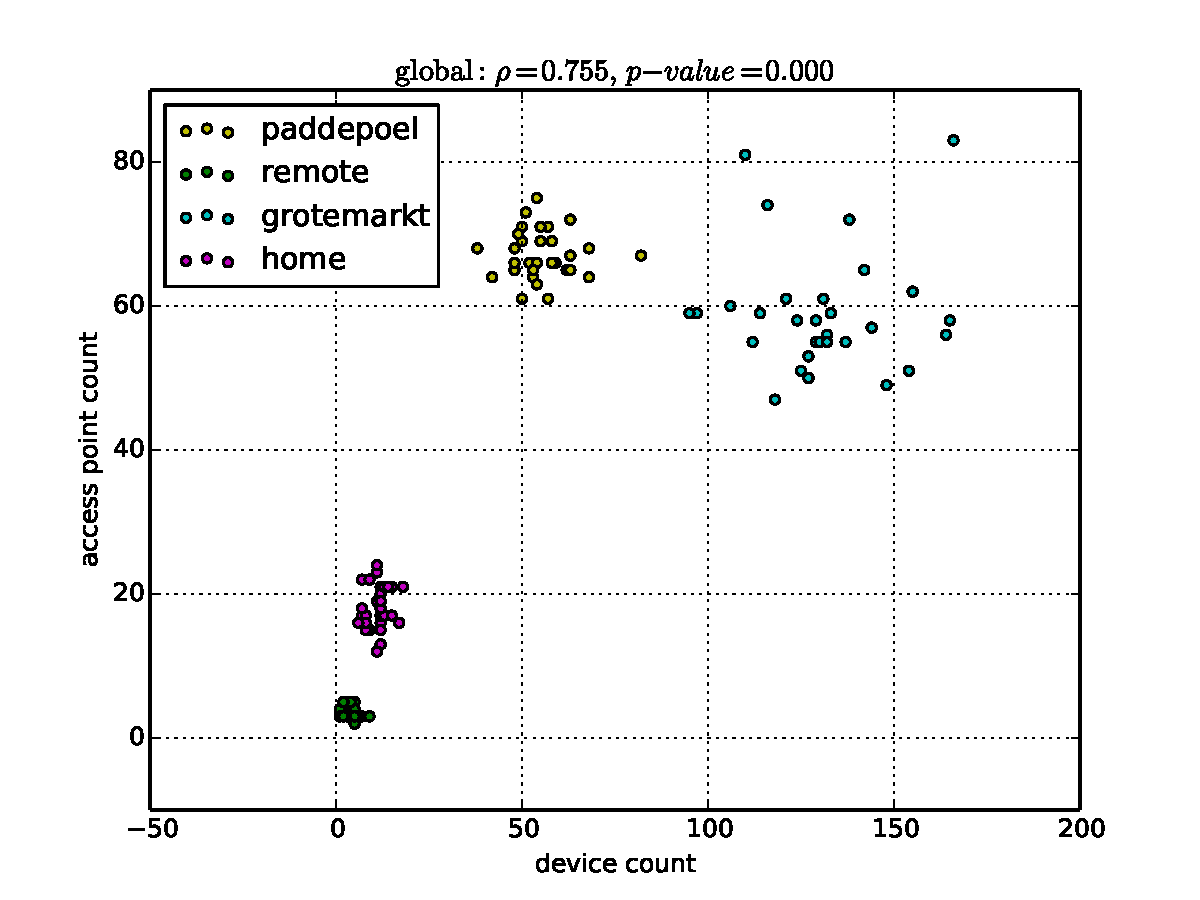
\includegraphics[width=0.7\textwidth]{./img/result/day/day2/global-pr-vs-ap}
    }
  }\\
  \subfloat[day 3]{
    \label{fig:ap-dc-day3}{
      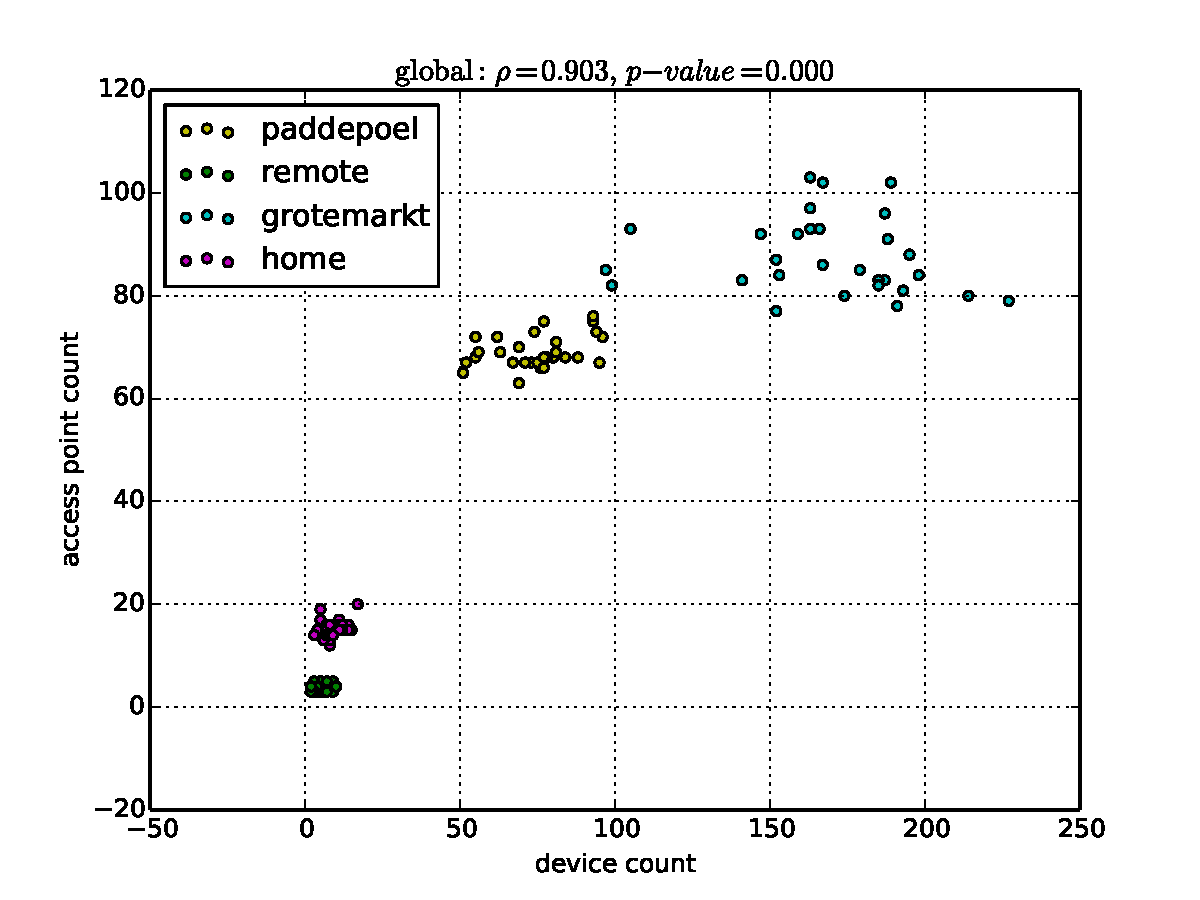
\includegraphics[width=0.7\textwidth]{./img/result/day/day3/global-pr-vs-ap}
    }
  }
  \subfloat[day 4]{
    \label{fig:ap-dc-day4}{
      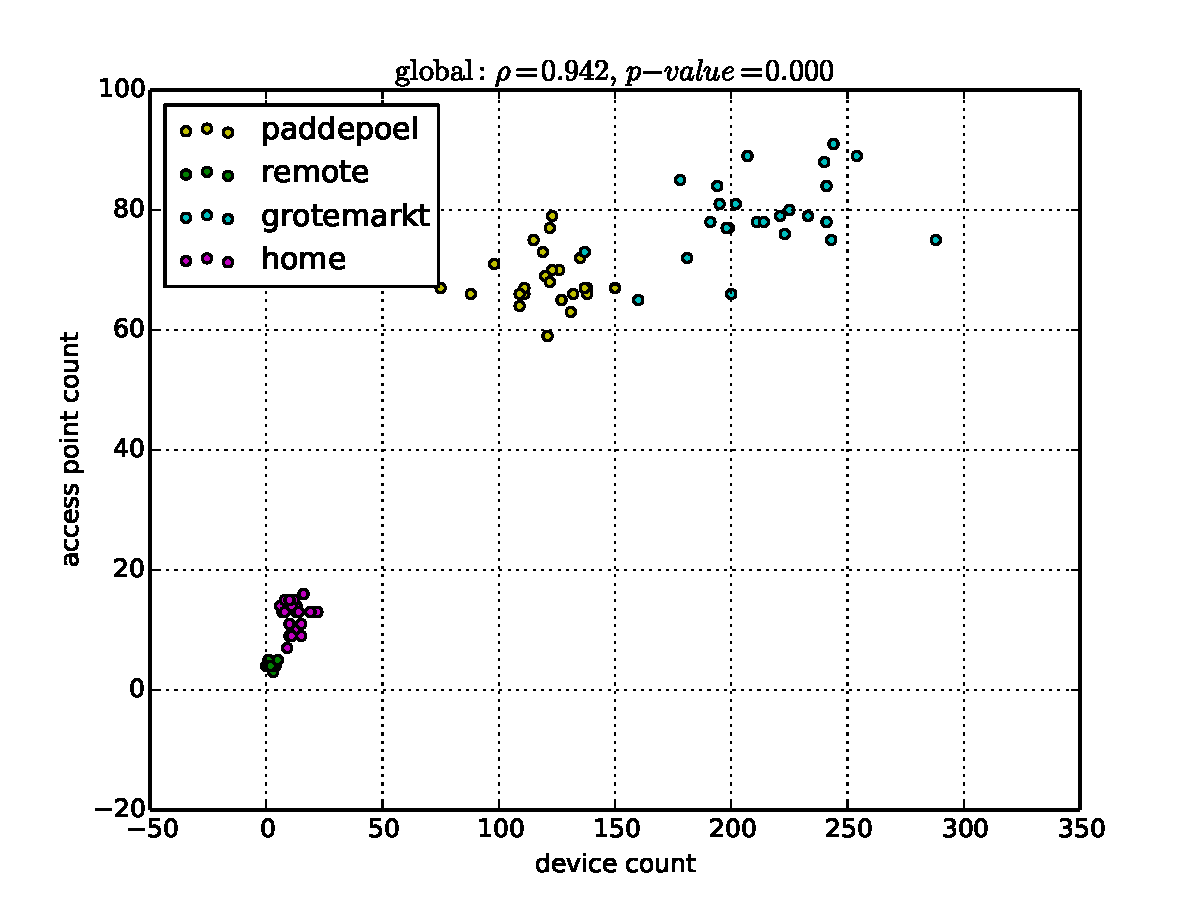
\includegraphics[width=0.7\textwidth]{./img/result/day/day4/global-pr-vs-ap}
    }
  }
  \end{adjustwidth}
  \caption[The scatter plots of the correlation between device count and \ac{AP}.]
  {The scatter plots showing the correlation between device count and \ac{AP} count in four days of experiment. The location is coded in color.}
  \label{fig:ap-dc-scatterplot}
\end{figure}

% ap vs device count
\begin{figure}[H]
  \begin{adjustwidth}{-1cm}{}
  \centering
  \subfloat[day 1]{
    \label{fig:hc-dc-day1}{
      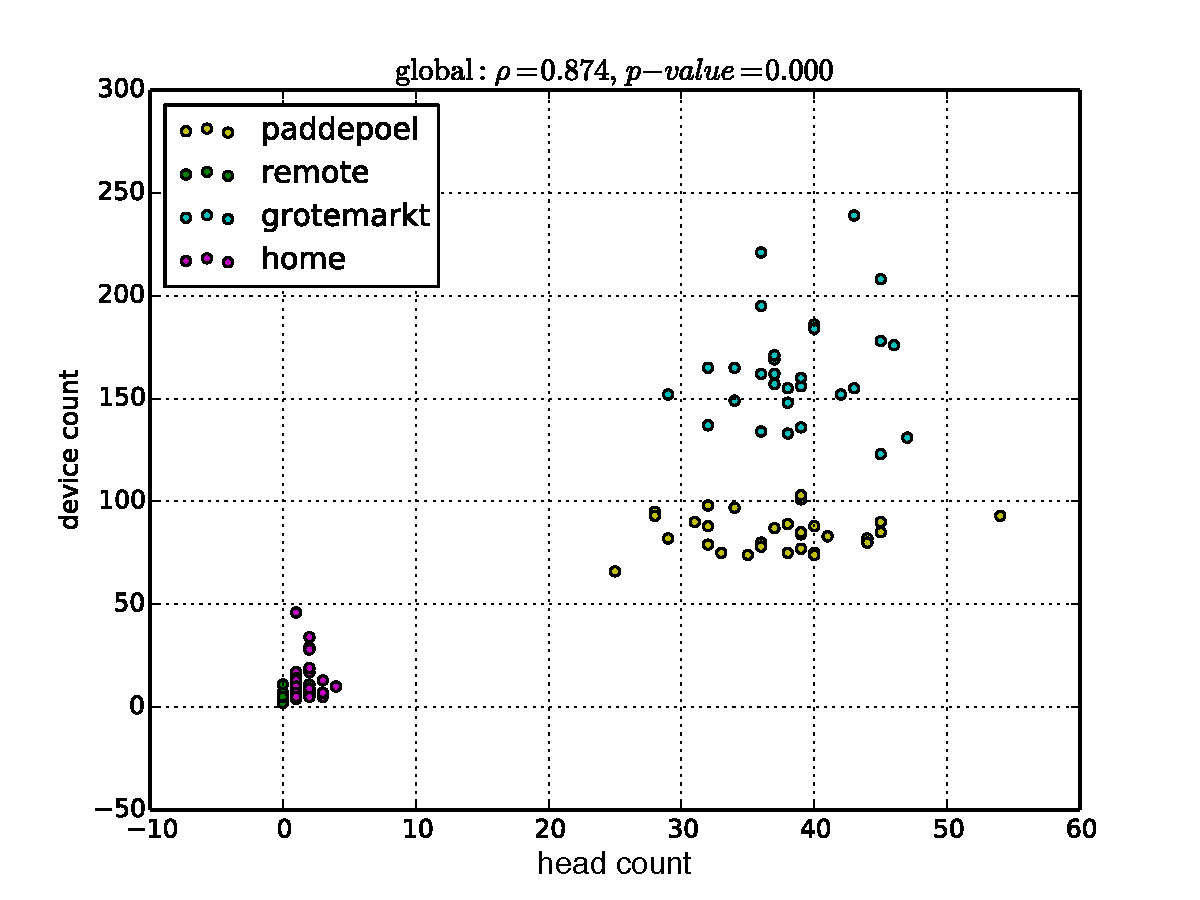
\includegraphics[width=0.7\textwidth]{./img/result/day/day1/global-gt-vs-pr}
    }
  }
  \subfloat[day 2]{
    \label{fig:hc-dc-day2}{
      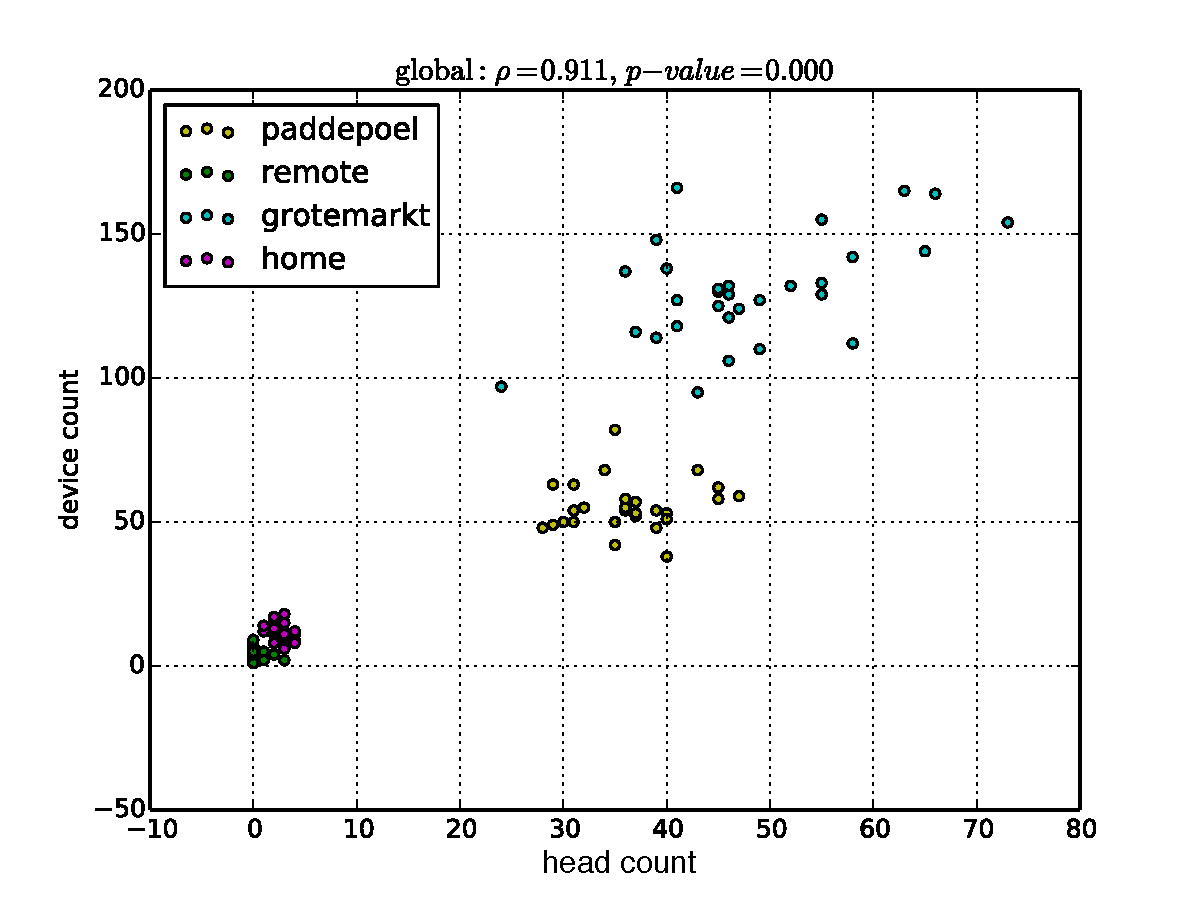
\includegraphics[width=0.7\textwidth]{./img/result/day/day2/global-gt-vs-pr}
    }
  }\\
  \subfloat[day 3]{
    \label{fig:hc-dc-day3}{
      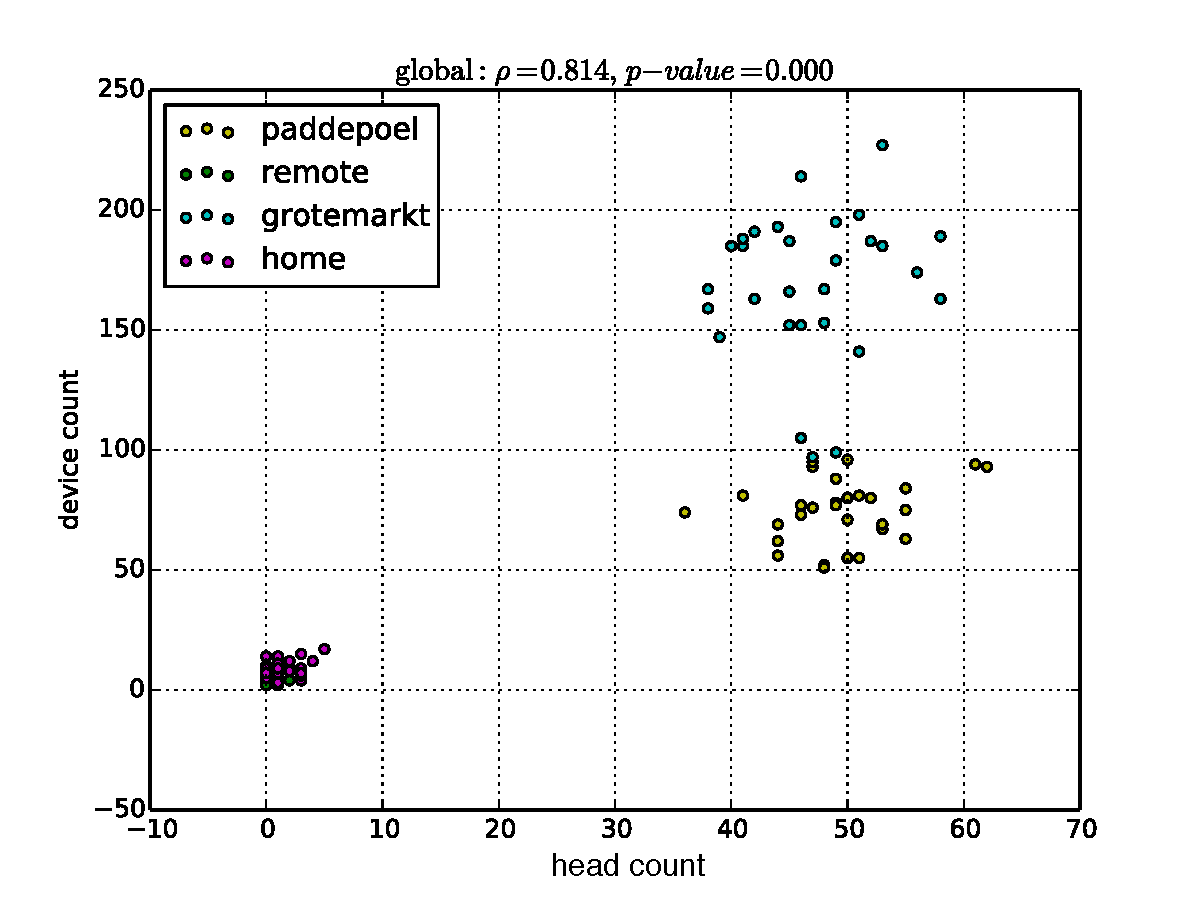
\includegraphics[width=0.7\textwidth]{./img/result/day/day3/global-gt-vs-pr}
    }
  }
  \subfloat[day 4]{
    \label{fig:hc-dc-day4}{
      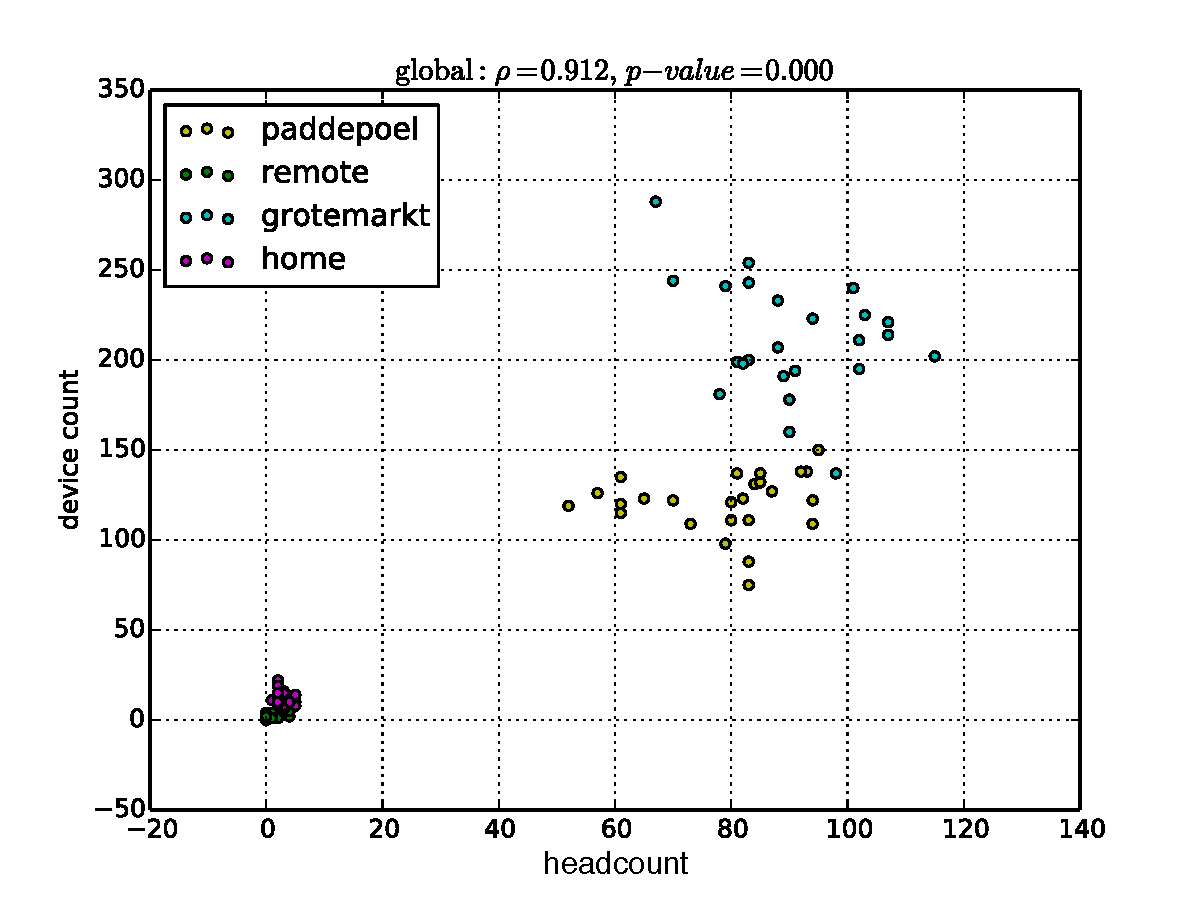
\includegraphics[width=0.7\textwidth]{./img/result/day/day4/global-gt-vs-pr}
    }
  }
  \end{adjustwidth}
  \caption[The scatter plots of the correlation between device count and \ac{AP} count.]
  {The scatter plots showing the correlation between device count and \ac{AP} count in four days of experiment. The location is coded in color.}
  \label{fig:hc-dc-scatterplot}
\end{figure}







\section{Line charts} % (fold)
\label{sec:line_charts}

\begin{figure}[H]
  \begin{adjustwidth}{-5cm}{}
  \centering
  \subfloat[day 1]{
    \label{fig:remote-day1}{
      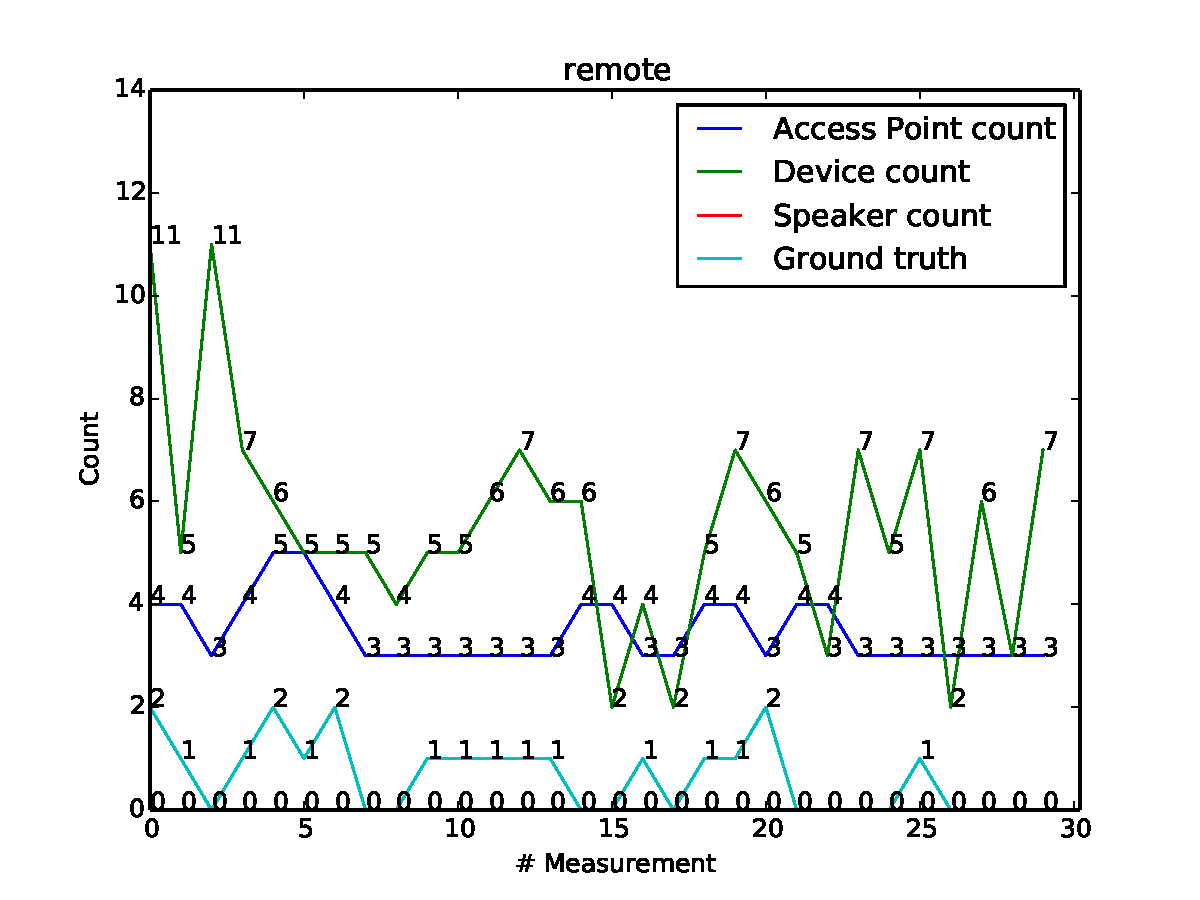
\includegraphics[width=0.7\textwidth]{./img/result/day/day1/remote-20161026}
    }
  }
  \subfloat[day 2]{
    \label{fig:remote-day2}{
      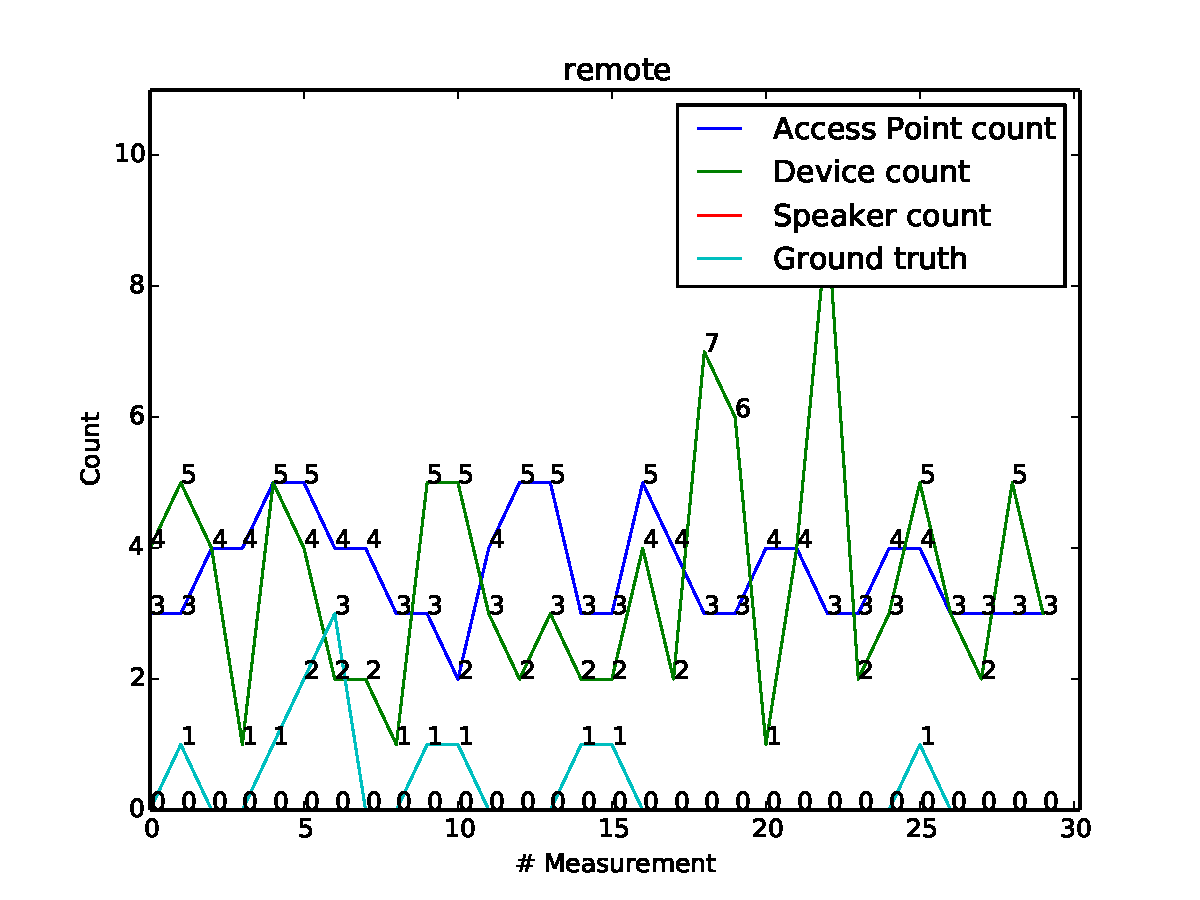
\includegraphics[width=0.7\textwidth]{./img/result/day/day2/remote-20161027}
    }
  }\\
  \subfloat[day 3]{
    \label{fig:remote-day3}{
      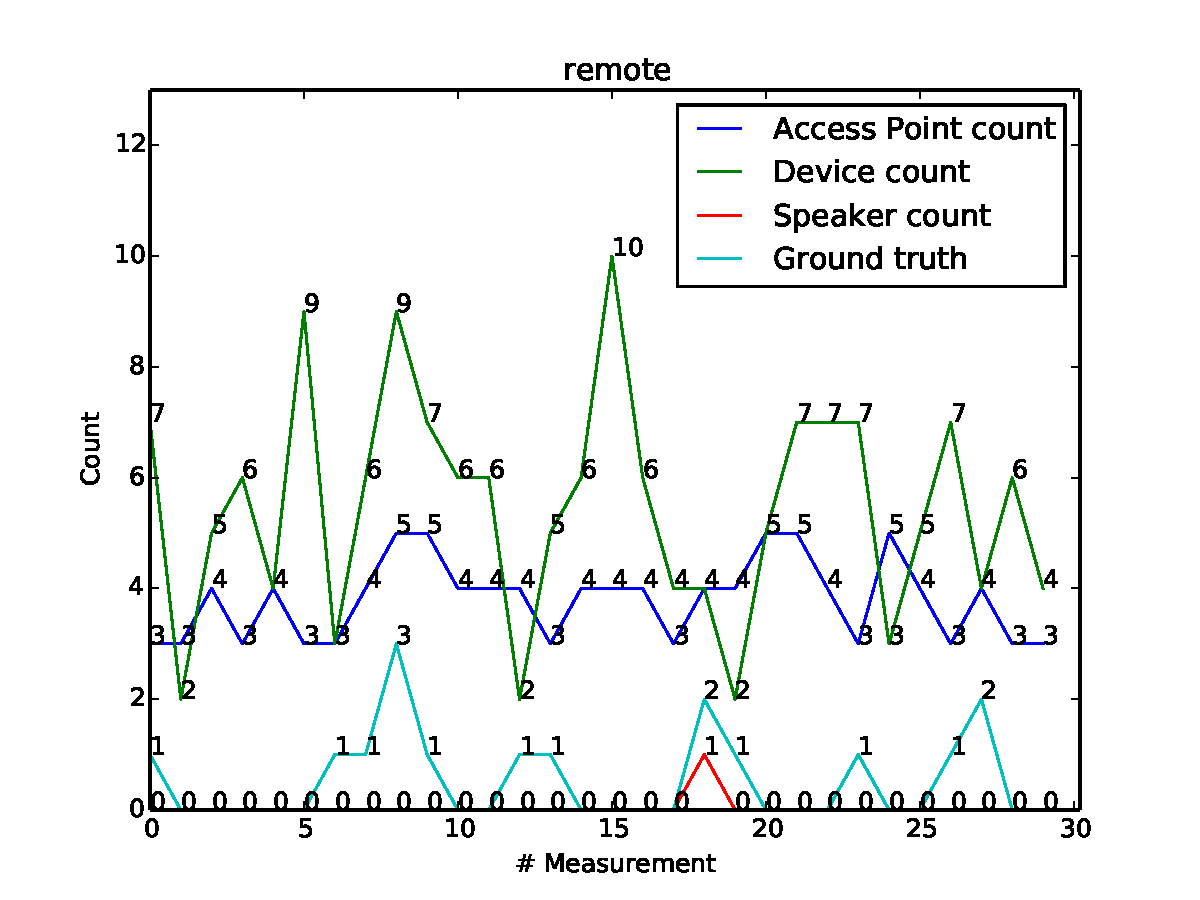
\includegraphics[width=0.7\textwidth]{./img/result/day/day3/remote-20161028}
    }
  }
  \subfloat[day 4]{
    \label{fig:remote-day4}{
      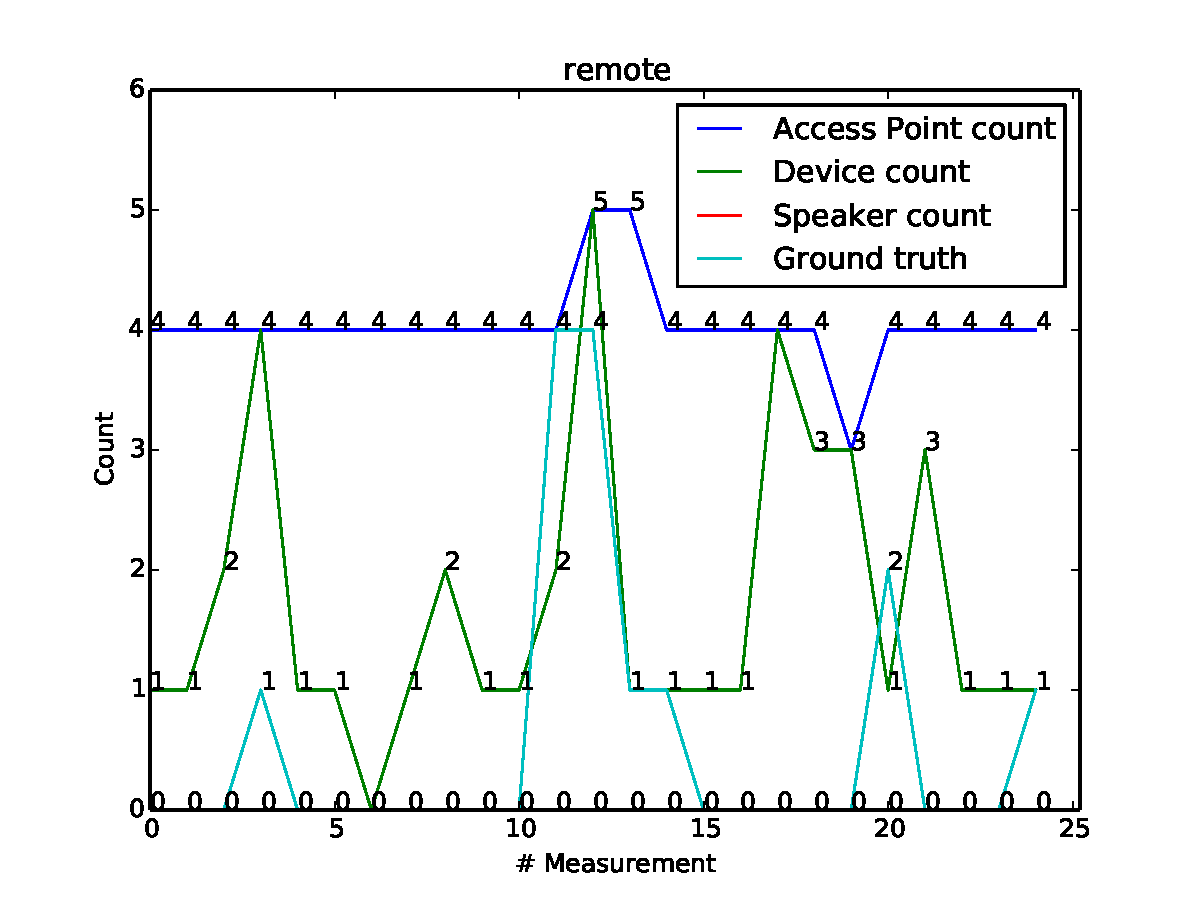
\includegraphics[width=0.7\textwidth]{./img/result/day/day4/remote-20161029}
    }
  }
  \end{adjustwidth}
  \caption[The line chart of sensor readings at remote area.]
  {The line chart of sensor readings at \textit{remote area} in four days of experiment.}
  \label{fig:result-remote-line-chart}
\end{figure}


\begin{figure}[H]
  \begin{adjustwidth}{-1cm}{}
  \centering
  \subfloat[day 1]{
    \label{fig:home-day1}{
      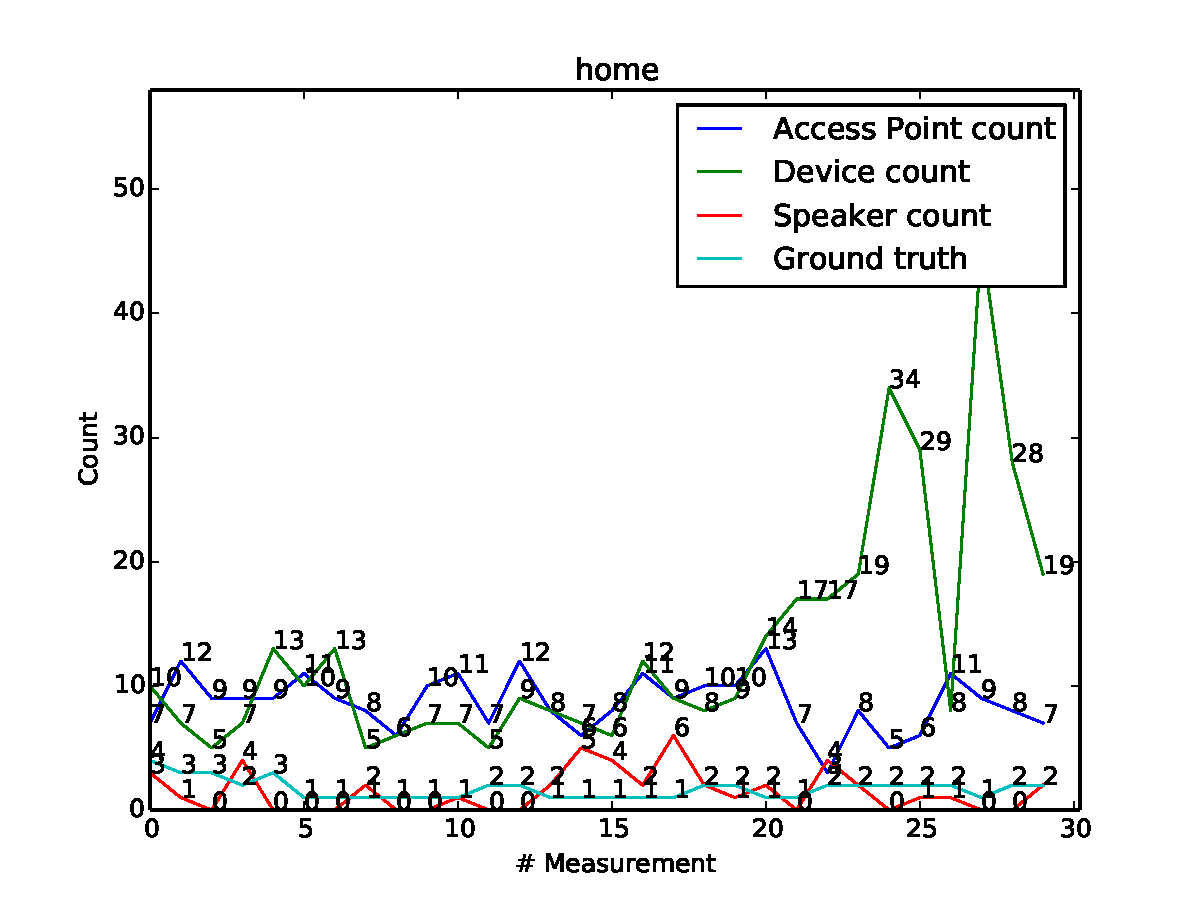
\includegraphics[width=0.7\textwidth]{./img/result/day/day1/home-20161026}
    }
  }
  \subfloat[day 2]{
    \label{fig:home-day2}{
      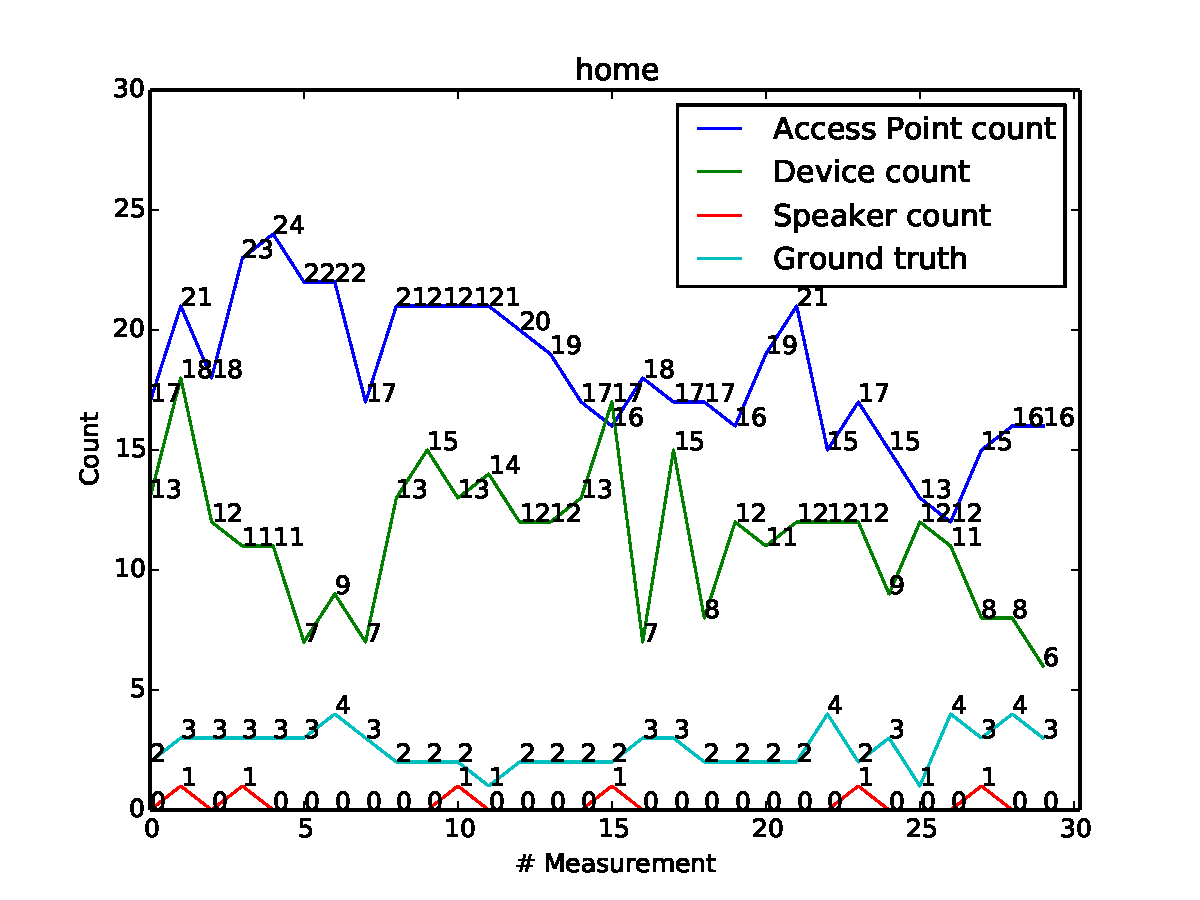
\includegraphics[width=0.7\textwidth]{./img/result/day/day2/home-20161027}
    }
  }\\
  \subfloat[day 3]{
    \label{fig:home-day3}{
      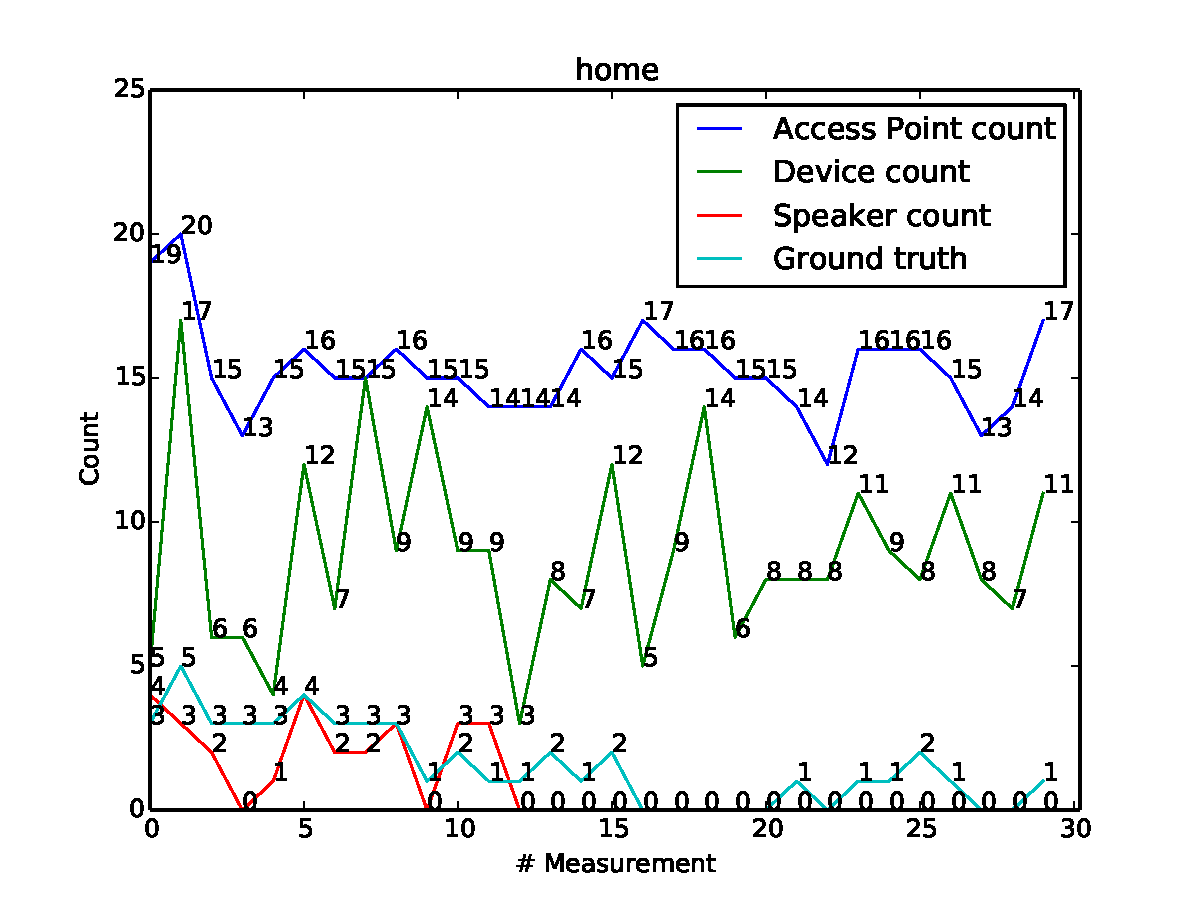
\includegraphics[width=0.7\textwidth]{./img/result/day/day3/home-20161028}
    }
  }
  \subfloat[day 4]{
    \label{fig:home-day4}{
      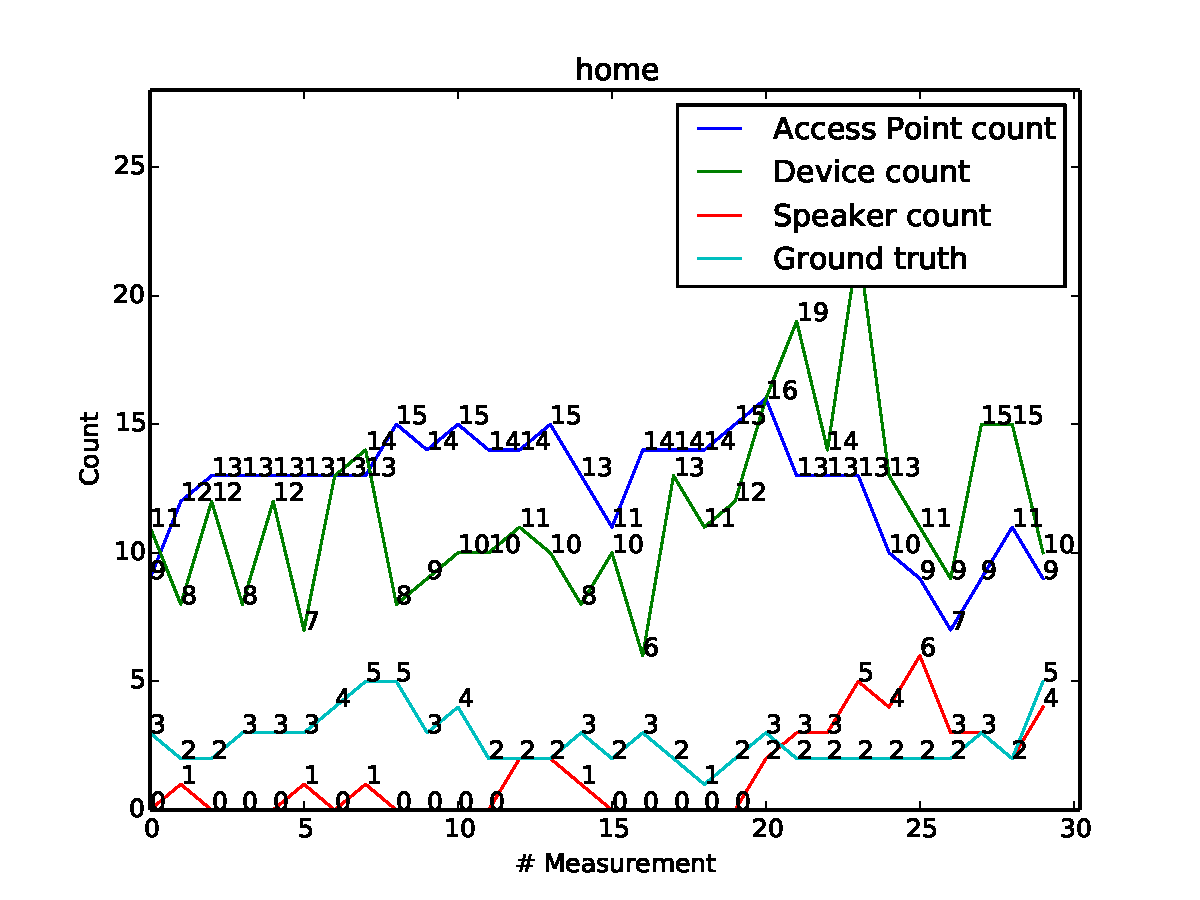
\includegraphics[width=0.7\textwidth]{./img/result/day/day4/home-20161029}
    }
  }
  \end{adjustwidth}
  \caption[The line chart of sensor readings at home.]
  {The line chart of sensor readings at \textit{home} in four days of experiment.}
  \label{fig:result-home-line-chart}
\end{figure}


\begin{figure}[H]
  \begin{adjustwidth}{-5cm}{}
  \centering
  \subfloat[day 1]{
    \label{fig:paddepoel-day1}{
      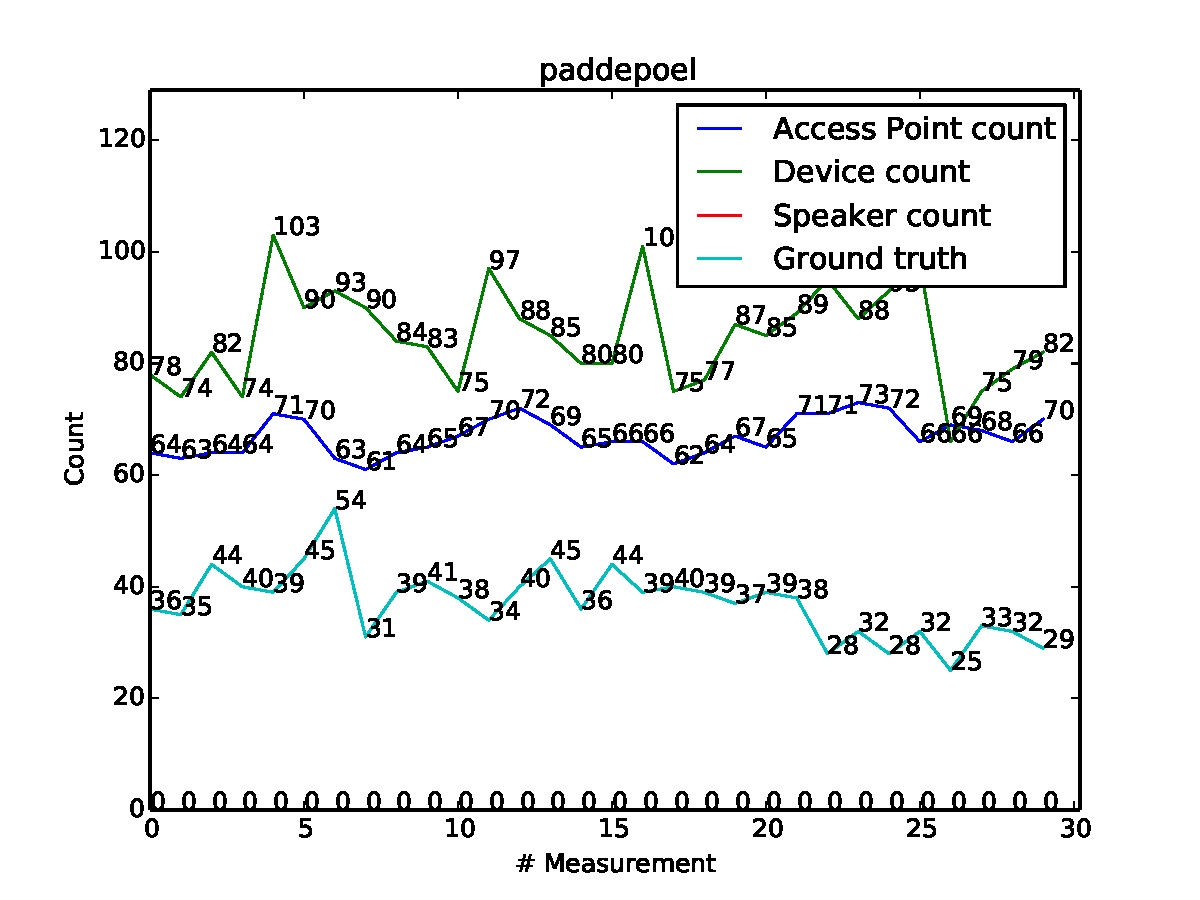
\includegraphics[width=0.7\textwidth]{./img/result/day/day1/paddepoel-20161026}
    }
  }
  \subfloat[day 2]{
    \label{fig:paddepoel-day2}{
      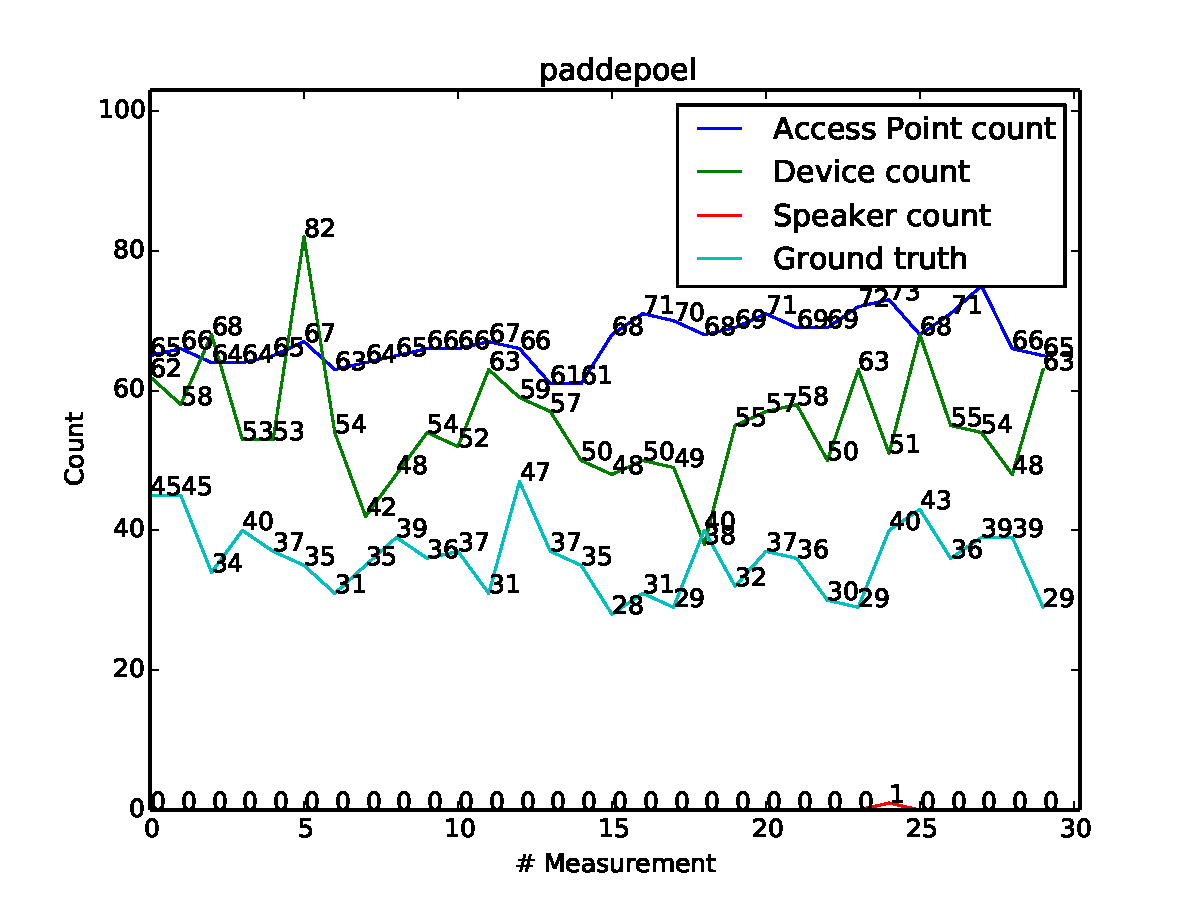
\includegraphics[width=0.7\textwidth]{./img/result/day/day2/paddepoel-20161027}
    }
  }\\
  \subfloat[day 3]{
    \label{fig:paddepoel-day3}{
      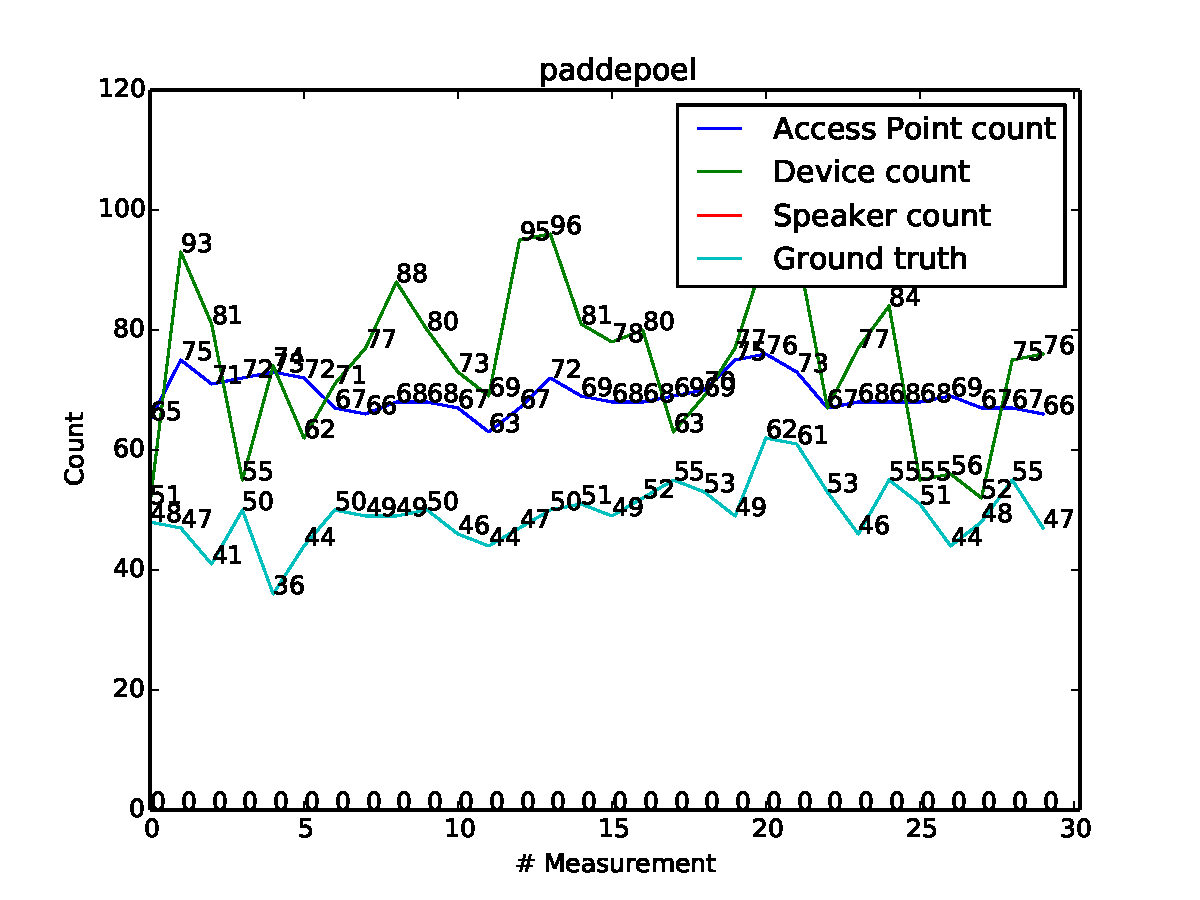
\includegraphics[width=0.7\textwidth]{./img/result/day/day3/paddepoel-20161028}
    }
  }
  \subfloat[day 4]{
    \label{fig:paddepoel-day4}{
      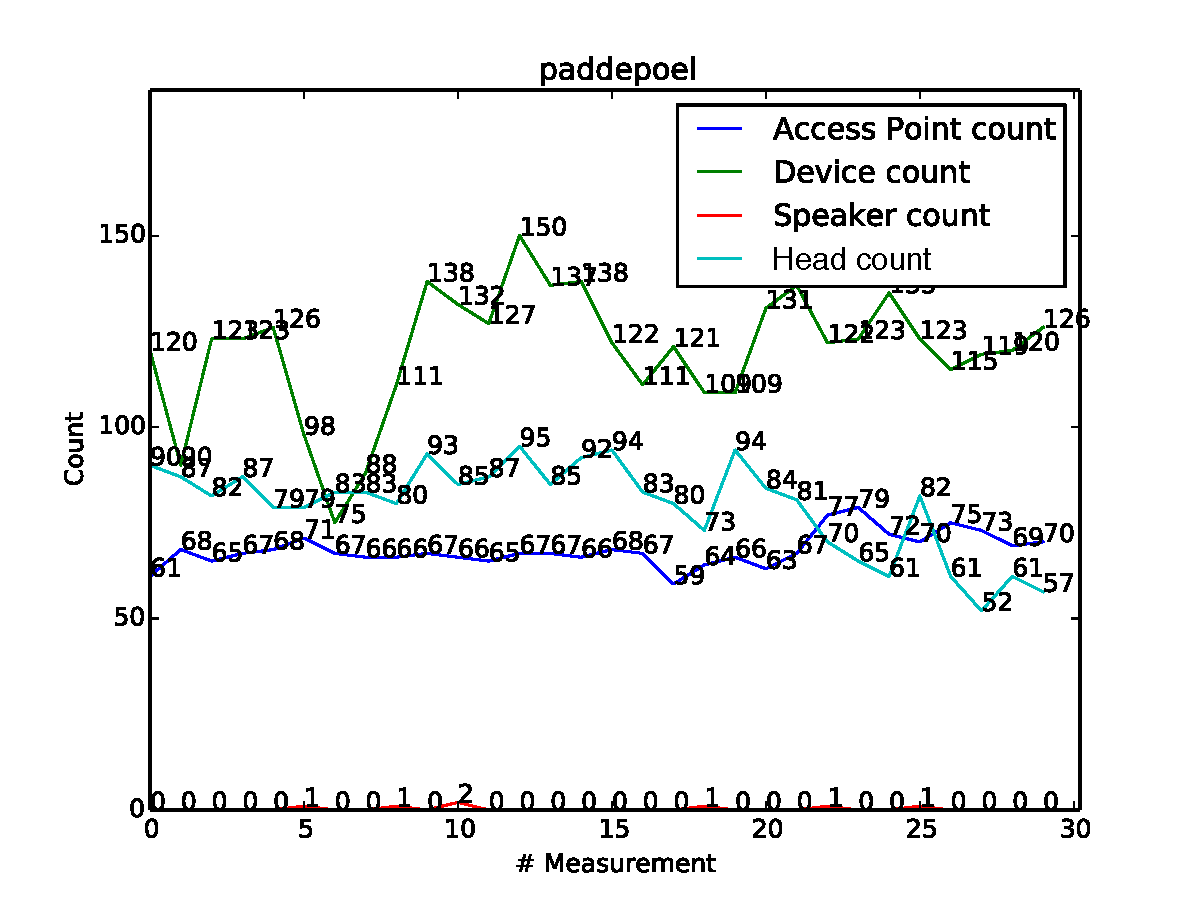
\includegraphics[width=0.7\textwidth]{./img/result/day/day4/paddepoel-20161029}
    }
  }
  \end{adjustwidth}
  \caption[The line chart of sensor readings at Paddepoel Shopping Center.]
  {The line chart of sensor readings at \textit{Paddepoel Shopping Center} in four days of experiment.}
  \label{fig:result-paddepoel-line-chart}
\end{figure}


\begin{figure}[H]
  \begin{adjustwidth}{-2cm}{}
  \centering
  \subfloat[day 1]{
    \label{fig:grotemarkt-day1}{
      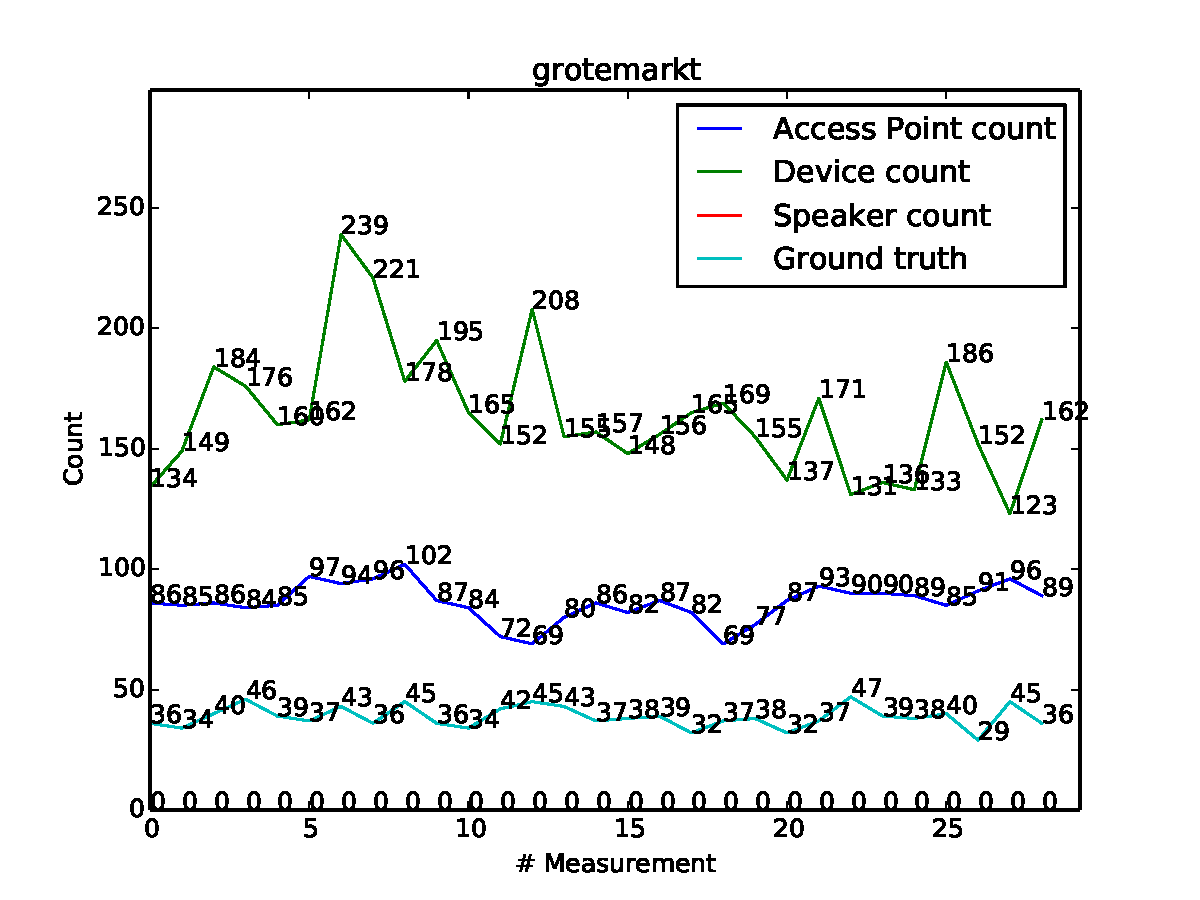
\includegraphics[width=0.7\textwidth]{./img/result/day/day1/grotemarkt-20161026}
    }
  }
  \subfloat[day 2]{
    \label{fig:grotemarkt-day2}{
      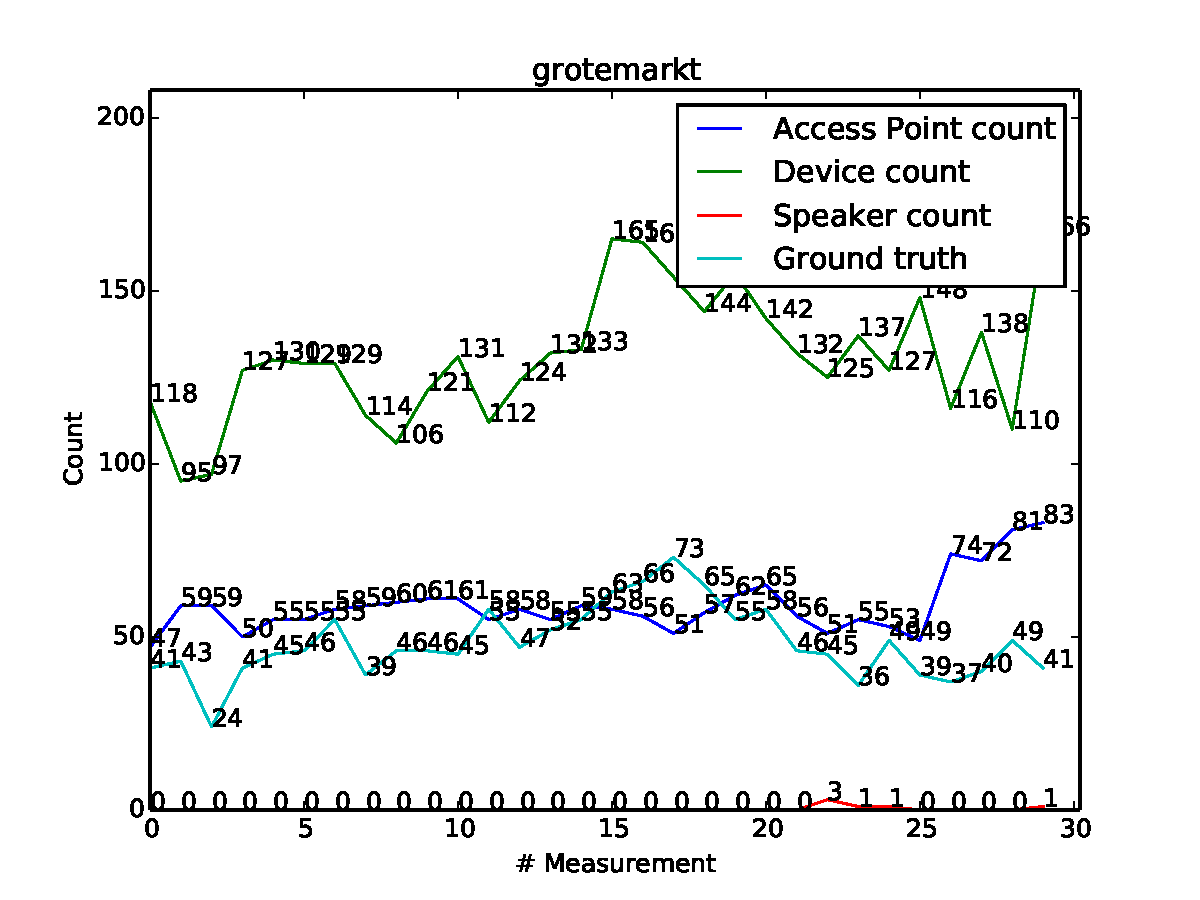
\includegraphics[width=0.7\textwidth]{./img/result/day/day2/grotemarkt-20161027}
    }
  }\\
  \subfloat[day 3]{
    \label{fig:grotemarkt-day3}{
      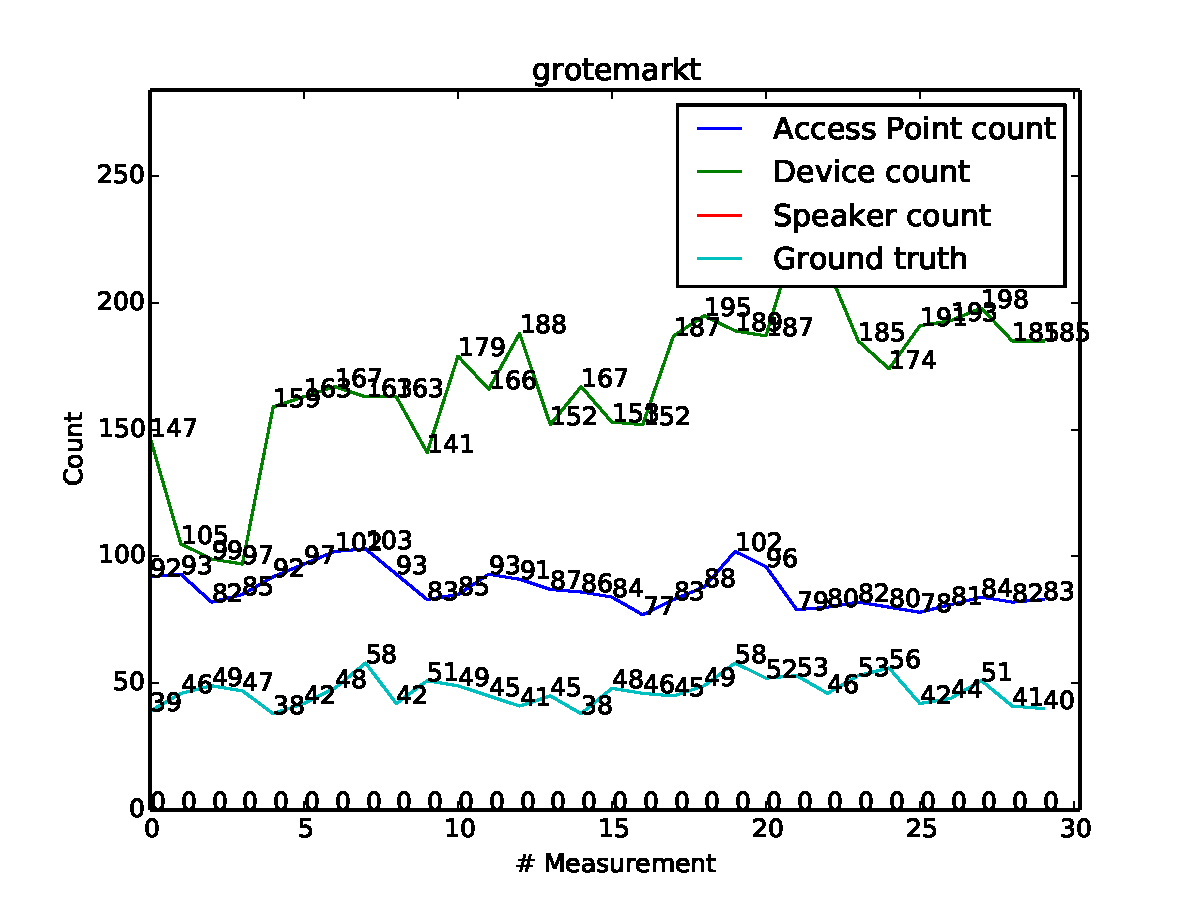
\includegraphics[width=0.7\textwidth]{./img/result/day/day3/grotemarkt-20161028}
    }
  }
  \subfloat[day 4]{
    \label{fig:grotemarkt-day4}{
      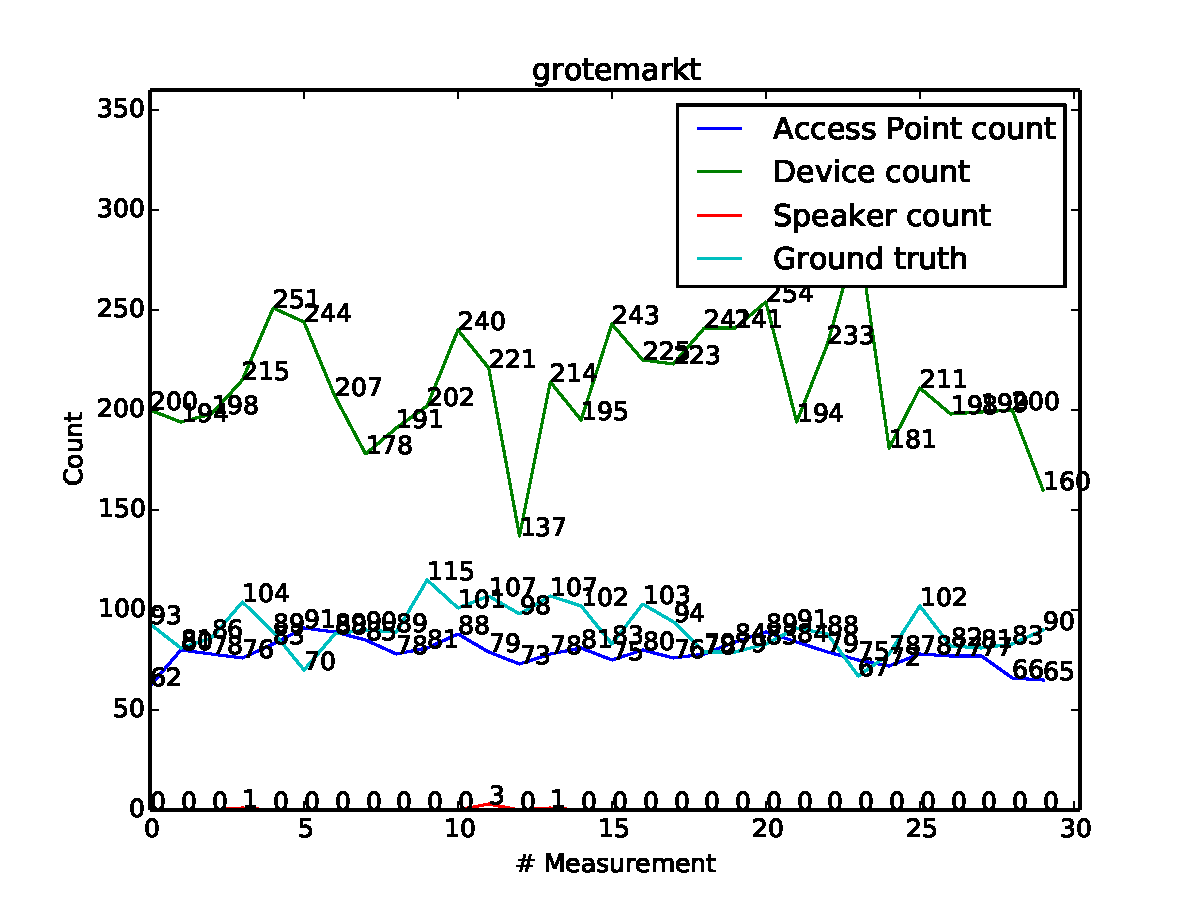
\includegraphics[width=0.7\textwidth]{./img/result/day/day4/grotemarkt-20161029}
    }
  }
  \end{adjustwidth}
  \caption[The line chart of sensor readings at Grote Markt.]
  {The line chart of sensor readings at \textit{Grote Markt} in four days of experiment.}
  \label{fig:result-grotemarkt-line-chart}
\end{figure}
=======
\chapter{Appendix Test}
Lorem ipsum at nusquam appellantur his, ut eos erant homero
concludaturque. Albucius appellantur deterruisset id eam, vivendum
partiendo dissentiet ei ius. Vis melius facilisis ea, sea id convenire
referrentur, takimata adolescens ex duo. Ei harum argumentum per. Eam
vidit exerci appetere ad, ut vel zzril intellegam interpretaris.
\graffito{More dummy text.}

%Errem omnium ea per, pro congue populo ornatus cu, ex qui dicant
%nemore melius. No pri diam iriure euismod. Graecis eleifend
%appellantur quo id. Id corpora inimicus nam, facer nonummy ne pro,
%kasd repudiandae ei mei. Mea menandri mediocrem dissentiet cu, ex
%nominati imperdiet nec, sea odio duis vocent ei. Tempor everti
%appareat cu ius, ridens audiam an qui, aliquid admodum conceptam ne
%qui. Vis ea melius nostrum, mel alienum euripidis eu.

\section{Appendix Section Test}
Test: \autoref{tab:moreexample} (This reference should have a 
lowercase, small caps \spacedlowsmallcaps{A} if the option 
\texttt{floatperchapter} is activated, just as in the table itself
 $\rightarrow$ however, this does not work at the moment.)

\begin{table}[h]
    \myfloatalign
  \begin{tabularx}{\textwidth}{Xll} \toprule
    \tableheadline{labitur bonorum pri no} & \tableheadline{que vista}
    & \tableheadline{human} \\ \midrule
    fastidii ea ius & germano &  demonstratea \\
    suscipit instructior & titulo & personas \\
    %postulant quo & westeuropee & sanctificatec \\
    \midrule
    quaestio philosophia & facto & demonstrated \\
    %autem vulputate ex & parola & romanic \\
    %usu mucius iisque & studio & sanctificatef \\
    \bottomrule
  \end{tabularx}
  \caption[Autem usu id]{Autem usu id.}
  \label{tab:moreexample}
\end{table}

%Nulla fastidii ea ius, exerci suscipit instructior te nam, in ullum
%postulant quo. Congue quaestio philosophia his at, sea odio autem
%vulputate ex. Cu usu mucius iisque voluptua. Sit maiorum propriae at,
%ea cum primis intellegat. Hinc cotidieque reprehendunt eu nec. Autem
%timeam deleniti usu id, in nec nibh altera.




\section{Another Appendix Section Test}
Equidem detraxit cu nam, vix eu delenit periculis. Eos ut vero
constituto, no vidit propriae complectitur sea. Diceret nonummy in
has, no qui eligendi recteque consetetur. Mel eu dictas suscipiantur,
et sed placerat oporteat. At ipsum electram mei, ad aeque atomorum
mea. There is also a useless Pascal listing below: \autoref{lst:useless}.

\begin{lstlisting}[float=b,language=Pascal,frame=tb,caption={A floating example (\texttt{listings} manual)},label=lst:useless]
for i:=maxint downto 0 do
begin
{ do nothing }
end;
\end{lstlisting}

%Ei solet nemore consectetuer nam. Ad eam porro impetus, te choro omnes
%evertitur mel. Molestie conclusionemque vel at, no qui omittam
%expetenda efficiendi. Eu quo nobis offendit, verterem scriptorem ne
%vix.
>>>>>>> deb4eee798046ff3050e2fdc49aff179daa28237

